% COMP550 progress report, due Dec 6 2026. ACL style (final mode, no line numbers).
% Build: sbatch report/build.sbatch   (pdflatex + bibtex on a compute node; never on the login node)
% Numbers: docs/results_seeds.md (3-seed tables). Longer prose: docs/progress_report.md.
\documentclass[11pt]{article}
\usepackage[final]{acl}
\usepackage{times}
\usepackage{latexsym}
\usepackage[T1]{fontenc}
\usepackage[utf8]{inputenc}
\usepackage{microtype}
\usepackage{inconsolata}
\usepackage{graphicx}
\usepackage{booktabs}
\usepackage{amsmath}
\usepackage{xcolor}
\usepackage{tikz}
\usetikzlibrary{positioning,arrows.meta,fit,calc}
\graphicspath{{../results/}}

\newcommand{\tauone}{$\tau{=}0.1$}
\newcommand{\tauthree}{$\tau{=}0.3$}
\newcommand{\taufive}{$\tau{=}0.5$}

\title{Chasing the Edge: Adaptive Difficulty Sampling for GRPO\\
\large COMP550 Progress Report}

\author{Eren Acar Basaran \and Turan Berke Yakarer}

\begin{document}
\maketitle

\begin{abstract}
\citet{zhang2025interplay} show that reinforcement learning (RL) with GRPO gives a small language model
genuinely new reasoning ability only when it trains on problems at its \emph{edge of competence}, and they
fix that edge at one difficulty band for the whole run. The edge moves as the model learns. We replace the
fixed band with samplers that choose the difficulty of every batch, keeping model, data, reward and compute
identical, and compare three objectives: maximise the share of informative gradient, maximise measured
learning speed, or maximise headroom. Headroom wins. A threshold sampler that moves up as soon as the
model solves more than 20\% of the current level newly solves $95.0\pm1.7$ of 204 hard problems the base
model never solved, against 48 for the paper's band; on the three hardest levels, which it never trained
on, it beats uniform sampling over all levels ($27.7$ vs $20.0$ of 102, $p=0.002$). A control that samples
the range it discovered uniformly recovers 81\% of the gain: the right range is most of the win, and the
adaptive sampler is what found it. The arm with the most informative gradient learns nothing new, and an
improvement-rate bandit fails because the level it trains rewards itself.
\end{abstract}

\section{Problem}
\label{sec:problem}

GRPO \citep{shao2024deepseekmath} samples a group of $G$ answers per problem and scores each answer against
its group: $A_i = (r_i - \bar r)/\mathrm{std}(r)$. If all $G$ answers are right, or all are wrong, every
advantage is zero and the problem contributes \emph{exactly no gradient}. For a problem with success rate
$p$, the chance that a group is informative is $1-p^G-(1-p)^G$; with our $G=6$ it is below 6\% at $p=0.01$
and above 80\% for $0.3\le p\le0.7$. What the model can learn from therefore depends on where it is
\emph{now}.

\citet{zhang2025interplay} train a 100M-parameter decoder from scratch on synthetic arithmetic problems
whose difficulty is the number of operations (op 2--20), then fine-tune it with GRPO under a strict
process-verified reward: every reasoning step and the final answer must be correct. Their central finding is
that RL produces new ability only when training sits at the model's edge, and they train on one band, op
11--14, chosen once.

But the edge moves. In our reproduction of the paper's run, levels the band never trains on become
learnable: averaged over two seeds, success at op 15 rises from 0 to 0.25 and at op 16 from 0 to 0.12 within
100 steps, while the band keeps spending its budget on op 11--14. \textbf{Our question is whether a sampler
that tracks the moving edge creates more new ability than the fixed band, or only more reliability on what
the model can already do, and which notion of ``the edge'' a sampler should aim for.}

So far we have (i) reproduced the paper's base model and fixed-band baseline; (ii) built and run four
adaptive samplers (three thresholds and a bandit) and three baselines for 1--3 seeds each (17 runs); and (iii) found that targeting
headroom wins, that most of its advantage comes from \emph{which range} it trains on, and that two
intuitive objectives fail for identifiable reasons.

\section{Related Work}
\label{sec:related}

\paragraph{Curricula and learning progress.} Ordering training data from easy to hard is old
\citep{bengio2009curriculum}; self-paced learning lets the learner choose examples by its current loss
\citep{kumar2010selfpaced}. Automatic curricula treat the choice of task as a bandit whose reward is
\emph{learning progress}, the change in performance on a task \citep{graves2017automated,
matiisen2019teacher}; \citet{portelas2020survey} survey the area. Our bandit arm is a direct instance of
this family, and our results identify a failure mode specific to it under GRPO (\S\ref{sec:bandit}).

\paragraph{Difficulty and data selection for RL on LLMs.} GRPO-style training of reasoning models
\citep{shao2024deepseekmath,deepseek2025r1} wastes compute on groups with uniform reward. DAPO
\citep{yu2025dapo} discards such groups and resamples (\emph{dynamic sampling}); online difficulty
filtering keeps problems of intermediate accuracy \citep{bae2025online}; adaptive curricula adjust target
difficulty from the reward signal \citep{shi2025adarft}. These methods mostly aim at gradient efficiency,
i.e.\ at $p\approx0.5$. We test that objective directly against a headroom objective and find that it is
the wrong target in our setting (\S\ref{sec:signal}).

\paragraph{Does RL create new ability?} \citet{yue2025doesrl} argue from pass@$k$ that RL mostly sharpens
what the base model can already do. \citet{zhang2025interplay} show, in a controlled synthetic setting,
that it can create new ability at the edge of competence. We use their setting, data generator
\citep{zhou2025gsminfinite} and metric (problems never solved before RL that are solved after), and ask how
the training distribution should move during the run.

\section{Methodology}
\label{sec:method}

\begin{figure}[t]
\centering
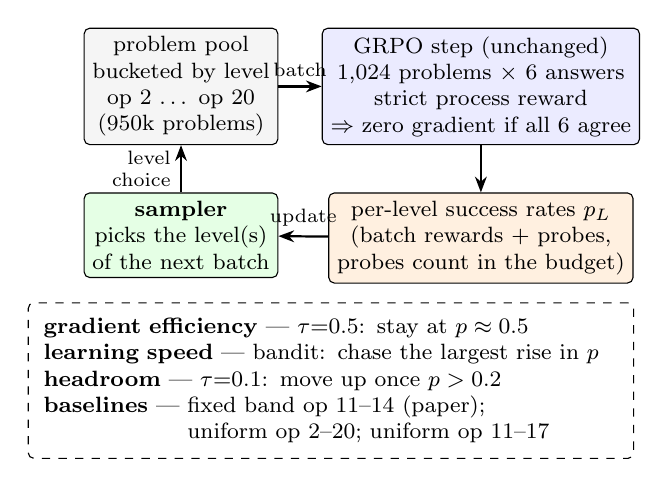
\begin{tikzpicture}[
  font=\footnotesize, >={Stealth[length=2mm]},
  box/.style={draw, rounded corners=2pt, align=center, inner sep=3pt, fill=#1},
  box/.default=white]
\node[box=gray!8, minimum width=2.3cm] (pool) {problem pool\\bucketed by level\\op 2 \dots\ op 20\\(950k problems)};
\node[box=blue!8, right=0.55cm of pool, minimum width=3.4cm] (grpo) {GRPO step (unchanged)\\1,024 problems $\times$ 6 answers\\strict process reward\\$\Rightarrow$ zero gradient if all 6 agree};
\node[box=orange!12, below=0.6cm of grpo, minimum width=3.4cm] (stats) {per-level success rates $p_L$\\(batch rewards + probes,\\probes count in the budget)};
\node[box=green!10, below=0.6cm of pool, minimum width=2.3cm] (sampler) {\textbf{sampler}\\picks the level(s)\\of the next batch};
\draw[->, thick] (pool) -- node[above, font=\scriptsize]{batch} (grpo);
\draw[->, thick] (grpo) -- (stats);
\draw[->, thick] (stats) -- node[above, font=\scriptsize]{update} (sampler);
\draw[->, thick] (sampler) -- node[left, font=\scriptsize, align=right]{level\\choice} (pool);
\node[below=0.35cm of $(sampler.south)!0.5!(stats.south)$, align=left, font=\footnotesize, text width=7.3cm] (rules) {%
\textbf{gradient efficiency} --- \taufive: stay at $p\approx0.5$\\
\textbf{learning speed} --- bandit: chase the largest rise in $p$\\
\textbf{headroom} --- \tauone: move up once $p>0.2$\\
\textbf{baselines} --- fixed band op 11--14 (paper);\\
\hphantom{\textbf{baselines} --- }uniform op 2--20; uniform op 11--17};
\node[draw, dashed, rounded corners=2pt, fit=(rules), inner sep=2pt] {};
\end{tikzpicture}
\caption{Overview. Only the sampler (green) differs between arms; the GRPO step, model, reward and budget
are identical. Each sampler turns the measured per-level success rates into the next batch's difficulty,
and each optimises a different notion of ``the edge''.}
\label{fig:overview}
\end{figure}

\paragraph{Setting.} We keep the paper's pretrained checkpoint (the 0.2/0.3/0.5 easy/medium/hard mixture of
its main experiment), data generator, GRPO hyper-parameters ($G=6$) and strict reward. Training runs in verl
\citep{sheng2025hybridflow} with vLLM generation \citep{kwon2023vllm}, unmodified: our samplers plug into
verl's curriculum-sampler hook, which chooses the dataset indices of every batch from a pre-generated pool
bucketed by level (Figure~\ref{fig:overview}). Every run gets the same budget, 100 steps of 1,024 problems
$\times$ 6 answers on one A40 (about 8.2 GPU-hours). Rollouts that adaptive samplers spend on probing
levels count against it.

\paragraph{Samplers.} \textbf{Threshold($\tau$)} trains one active level $L$, starting at op 11. It moves up
when the batch success rate exceeds $\tau+\delta$ for two consecutive steps and down when it falls below
$\max(\tau-\delta, \tau/2)$, with $\delta=0.1$; the clamp makes the lower bound reachable for $\tau=0.1$. In
a simulated model (success logistic in skill minus level) the rule ping-ponged between adjacent levels, which
straddle any band; we added a memory that never moves into a neighbour freshly measured on the wrong side.
We run $\tau\in\{0.1, 0.3, 0.5\}$. The \textbf{bandit} treats each level as an arm with reward
$r_L=p_L(t)-p_L(t-m)$, measured by probing every level every $m=25$ steps, value
$Q_L\leftarrow(1-\alpha)Q_L+\alpha r_L$ ($\alpha=0.3$) and $\varepsilon$-greedy selection ($\varepsilon=0.1$)
\citep{sutton2018rl}. \textbf{Controls:} the paper's fixed band (uniform over op 11--14), uniform over op
2--20 (``do harder problems help at all?''), and uniform over op 11--17 from step 0. The last one is the
range \tauone\ ended up visiting, chosen \emph{after} seeing its run; it separates the range from the
schedule.

\section{Experimental Evaluation}
\label{sec:eval}

\paragraph{Test sets and metrics.} Held-out sets, disjoint from the training pool: easy (op 2--10, 225
problems), medium (op 11--14, 800) and hard (op 15--20, 204). We draw 128 samples per problem at $T=0.7$ and
score with the paper's evaluation criterion. pass@1 measures reliability and pass@128 reachability, both
with the unbiased estimator \citep{chen2021codex}. \textbf{The headline metric is the paper's: problems the
base model never solved (0 of 128) that the trained model solves at least once.} The base model solves none
of the 204 hard problems, so on the hard set every solved problem is new. We also report the share of
training groups with a nonzero gradient, from the training logs.

\paragraph{Seeds and statistics.} Three training seeds for \tauone, uniform, the op 11--17 control and the
bandit; two for the fixed band and \tauthree; one for \taufive, which never leaves op 11. We report
mean $\pm$ SD over seeds. For paired comparisons the problem is the unit: per problem, the share of arm A's
seeds that newly solve it minus the share of B's; an exact two-sided sign test over problems with a nonzero
difference and a 95\% bootstrap CI (10,000 draws). Tests are not corrected for multiple comparisons.

\paragraph{Reproduction.} The base checkpoint reproduces the paper's base-model numbers (31 of 32
comparisons within six points; e.g.\ op 11--14 pass@128 41.8 vs.\ about 42), and the 1024-token answer
limit is not binding (correct solutions stay under 440 tokens). Our fixed-band run matches the paper's
released RL checkpoint within one point on every test set: medium pass@1 49.2 vs.\ 49.4, hard pass@128 23.5
vs.\ 23.5, and 48 of 204 hard problems newly solved for both, in both of our seeds. All comparisons below
are against this baseline.

\section{Preliminary Results}
\label{sec:results}

\begin{table*}[t]
\centering
\small
\begin{tabular}{lcccccc}
\toprule
& & \multicolumn{3}{c}{hard set, op 15--20} & op 18--20 & informative \\
\cmidrule(lr){3-5}
arm & seeds & pass@1 & pass@128 & \textbf{new} (/204) & \textbf{new} (/102) & groups \\
\midrule
threshold \tauone\ (headroom)        & 3 & $\mathbf{22.8\pm0.2}$ & $\mathbf{46.6\pm0.8}$ & $\mathbf{95.0\pm1.7}$ & $\mathbf{27.7\pm0.6}$ & 24.7\% \\
control: uniform op 11--17           & 3 & $20.4\pm0.2$ & $42.3\pm1.0$ & $86.3\pm2.1$ & $24.0\pm2.0$ & 28.6\% \\
uniform op 2--20                     & 3 & $16.8\pm0.5$ & $38.2\pm0.5$ & $78.0\pm1.0$ & $20.0\pm1.0$ & 18.8\% \\
fixed band op 11--14 (paper)         & 2 & $9.9\pm0.4$  & $23.5\pm0.0$ & $48.0\pm0.0$ & $6.0\pm0.0$  & 35.4\% \\
threshold \tauthree                  & 2 & $10.5\pm1.2$ & $23.8\pm1.7$ & $48.5\pm3.5$ & $4.0\pm1.4$  & 34.0\% \\
bandit, $m=25$ (learning speed)      & 3 & $8.5\pm1.3$  & $19.9\pm1.7$ & $40.7\pm3.5$ & $3.3\pm1.5$  & 29.1\% \\
threshold \taufive\ (gradient eff.)  & 1 & 0.0 & 0.0 & 0 & 0 & 40.1\% \\
\bottomrule
\end{tabular}
\caption{Main results (mean $\pm$ SD over seeds). ``New'' = newly solved: solved at least once in 128 samples
by the trained model and never by the base model. ``Informative groups'' = share of training groups with a
nonzero gradient over the run. Only uniform op 2--20 (16k groups per run) and, through $\varepsilon$-exploration, the bandit (5k) trained on op 18--20.}
\label{tab:main}
\end{table*}

\begin{figure*}[t]
\centering
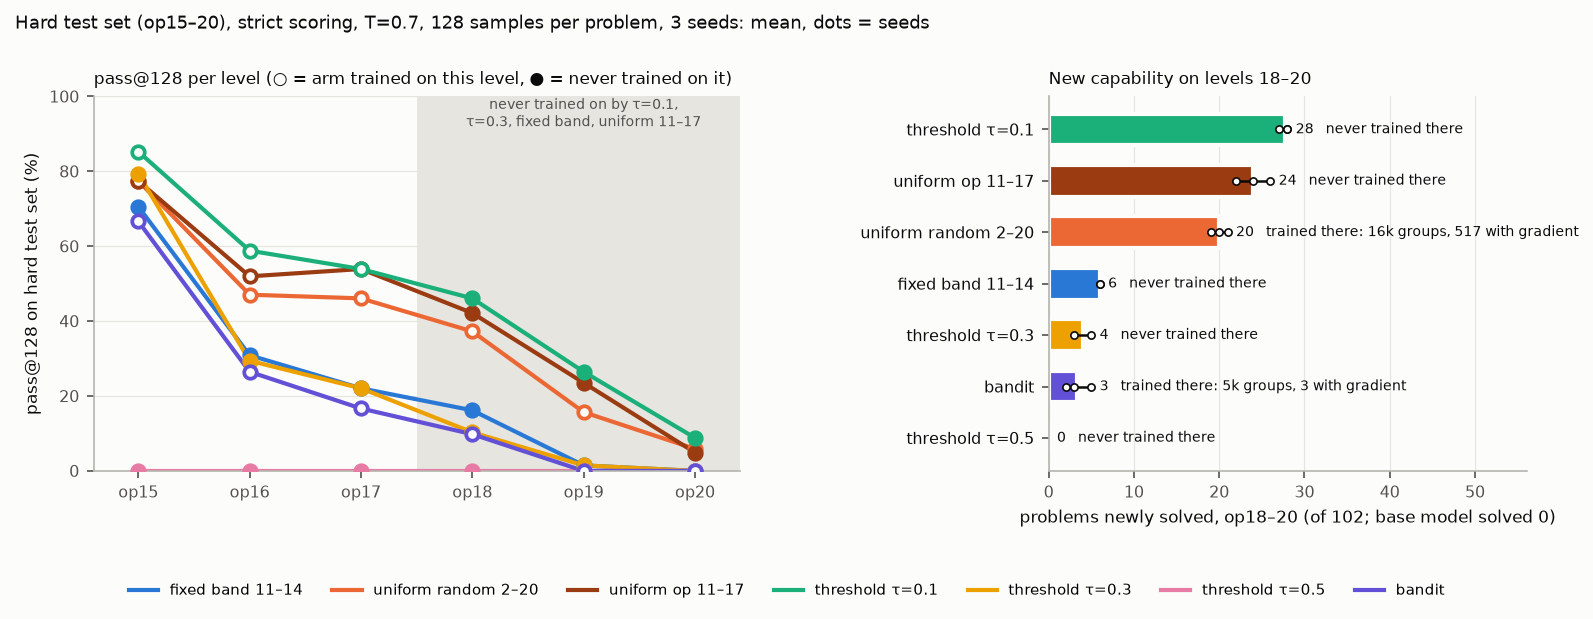
\includegraphics[width=\textwidth]{hard_by_level.png}
\caption{Hard test set by level. Left: pass@128 per level; hollow markers mark levels the arm trained on.
Right: problems newly solved on op 18--20, which \tauone\ and the op 11--17 control never trained on
(bars: mean over seeds; dots: seeds).}
\label{fig:hard}
\end{figure*}

Table~\ref{tab:main} summarises all arms. The samplers behaved the same way in every seed: \tauone\ climbed
from op 11 to op 14 by step 8, reached op 15 at step 16, op 16 at step 22--25 and op 17 at step 45--54, and
stayed there, its success rate hovering near 0.17, below the 0.2 move-up bound. \tauthree\ climbed through
the paper's band and stopped at op 14 by step 25. \taufive\ never left op 11. The bandit settled on op 12--14.

\subsection{Headroom: levels \texorpdfstring{\tauone}{tau=0.1} never trained on}

Neither \tauone\ nor the fixed band ever trained on op 18--20; uniform op 2--20 did, with 16\% of its
problems. Yet \tauone\ newly solves $27.7\pm0.6$ of those 102 problems and uniform $20.0\pm1.0$
(Figure~\ref{fig:hard}). Paired by problem over three seeds each, \tauone\ solves 15 problems more often and
uniform 2 ($p=0.002$; $+7.7$ per seed, 95\% CI $[+3.7, +12.3]$), and the direction holds in every seed
separately. The gradient explains it: 97\% of uniform's groups at op 18--20 had zero gradient, because every
answer there failed. \tauone\ instead put 84\% of its groups on op 15--17 while those levels were at the
edge (20,642 informative groups per run, vs.\ 2,300 for uniform and 0 for the fixed band), and the skill it
built carried two to three levels beyond anything it trained on.

\subsection{Range or schedule?}
\label{sec:range}

\tauone\ differs from the fixed band in two ways: it trains on a different range (op 11--17), and it visits
those levels in order. The op 11--17 control has the range without the schedule. Table~\ref{tab:decomp}
splits \tauone's gain over the fixed band into three steps.

\begin{table}[t]
\centering
\small
\begin{tabular}{lcc}
\toprule
step & hard ($+47.0$) & op 18--20 ($+21.7$) \\
\midrule
harder problems\textsuperscript{a} & $+30.0$ (64\%) & $+14.0$ (65\%) \\
right range\textsuperscript{b}     & $+8.3$ (18\%)  & $+4.0$ (18\%) \\
schedule\textsuperscript{c}        & $+8.7$ (18\%)  & $+3.7$ (17\%) \\
\bottomrule
\end{tabular}
\caption{Decomposition of \tauone's gain over the fixed band in newly solved problems per seed.
\textsuperscript{a}uniform op 2--20 $-$ fixed band; \textsuperscript{b}control op 11--17 $-$ uniform op
2--20; \textsuperscript{c}\tauone\ $-$ control.}
\label{tab:decomp}
\end{table}

\textbf{The range is most of the win.} The control recovers 81\% of \tauone's gain on the hard set and 83\%
on op 18--20. \textbf{The schedule adds a small margin}: on the hard set \tauone\ beats the control on 17
problems and loses on 5 ($p=0.017$; $+8.7$ per seed, CI $[+3.3,+14.3]$), ahead in every seed; on op 18--20
alone the gap ($+3.7$, 8 vs.\ 2 problems, $p=0.11$) is not significant. Per level, the margin sits at op 15
(29.0 vs.\ 26.3) and op 16 (20.0 vs.\ 17.7), the levels \tauone\ trained \emph{while they were at the edge};
at op 17, where both trained heavily, they tie (18.3 each).

\textbf{What the adaptive sampler contributes is the range itself.} The paper's band gets 48 hard problems;
the range \tauone\ found gets 86 sampled uniformly and 95 with its schedule. op 11--17 is the paper's band
plus three levels where the base model's success rate is exactly zero: nothing in the base model's
measurements points to them, and we would not have tried this range without \tauone. A sampler that follows
the edge finds the right range in one run instead of a sweep over ranges.

\subsection{More informative gradient did not mean more learning}
\label{sec:signal}

The $\tau$ sweep ranks the arms in reverse order of gradient efficiency. \taufive\ keeps 40.1\% of its groups
informative, the most of any arm, and newly solves nothing; \tauone\ keeps 24.7\% and newly solves 95.
\tauone\ did not receive more gradient; it received it in a different place.

Per-step success rates of each level during training trace an S-shaped curve. For every level that starts
at $p\approx0$ (fixed band and uniform runs, two seeds each, training reward, $T=1$), the steepest rise is at
$p\approx0.10$--$0.21$, and the curve flattens at a ceiling of $p\approx0.35$--$0.58$. This explains both ends
of the sweep. \tauone's band $[0.05, 0.2]$ contains the steepest point: it trains each level during its
fastest improvement and moves on as the curve flattens. \taufive's band $[0.4, 0.6]$ is the ceiling: it
maximises informative groups where nothing is left to learn, and since op 11 levels off at 0.57, below the
0.6 move-up bound, it never leaves. Our proposal assumed $p=0.5$ was the sweet spot; under this reward and
temperature it is the end of a level's learning curve, not its midpoint. Values of $\tau$ between 0.1 and 0.3
are untested.

\subsection{The bandit rewards itself}
\label{sec:bandit}

The bandit is the weakest trained arm, below the fixed band in all three seeds ($40.7\pm3.5$ vs.\ 48). Its
reward is a level's improvement between probes, and the level it trains improves \emph{because} it is trained:
the greedy choice pays for itself, takes 90\% of every batch, and stays on op 12--14. op 15 became learnable
through spill-over anyway (probe success 0.10--0.31 by step 50 across seeds) and reached second place in
value, but under an argmax second place gets nothing: after the first value update, op 15+ received exactly
the $\varepsilon$ floor of 3.2\% of prompts in all three seeds. Probing every 10 steps instead of 25 made it
worse: the bandit locked on sooner, onto an easier level (op 12). Measurement lag aggravates the failure, but
self-reward causes it. We read this as a structural limitation of learning-progress curricula
\citep{graves2017automated,matiisen2019teacher} when the learner's own training produces the progress signal.

\subsection{Cost: reliability on easier problems}

\tauone's gain comes with a small, consistent loss of reliability on easier problems. Its easy pass@1 is
$83.9\pm0.2$, against $85.3\pm0.1$ for the control, 85.4 for the fixed band and 85.5 for the base model;
medium pass@1 is $46.7\pm0.4$ against 49.1 (control) and 49.2 (fixed band). This is not seed noise: every
cross-seed pair (6/6 vs.\ the fixed band, 9/9 vs.\ the control) has \tauone\ lower, and paired by problem the
easy deficit against the base model is $-1.6$ points (CI $[-3.0,-0.3]$). Reachability is unchanged: easy
pass@128 is 98.5 for \tauone, uniform and the control. The control, which keeps 57\% of its batch on op
11--14, has no such cost. If the right range is known, sampling it uniformly gets 81\% of the gain at no
reliability cost; \tauone\ finds the range and adds a small margin on the hardest problems.

\section{Limitations and Plan}
\label{sec:plan}

\paragraph{Limitations.} Runs are 100 steps, half the paper's length; the fixed band might catch up. Seeds
are 1--3 per arm (the fixed band's two seeds agree exactly, 48 and 48). The control's range was chosen in
hindsight, so 81\% is an upper bound on what a range picked in advance would achieve. Tests are uncorrected:
\tauone\ vs.\ uniform ($p=0.002$) survives any reasonable correction, \tauone\ vs.\ the control on the hard
set ($p=0.017$) is borderline. One model and one task family.

\paragraph{Plan for the final report.} (1) $\tau=0.15$ and $0.2$, which train inside the predicted peak
(needs $\delta=0.05$); (2) range-finding as a method: a short \tauone\ burn-in, then uniform sampling over
the range it found; (3) 200-step runs of \tauone, the control and the fixed band; (4) bandit fixes that
remove the self-reward loop (credit only improvement an arm did not train for, or mix in a headroom term);
(5) keeping a share of op 11--14 in \tauone's batches to remove the reliability cost.

\paragraph{Compute.} The 17 completed runs took 139 GPU-hours; the project total, including evaluation,
a bandit ablation and 48 GPU-hours lost to jobs that hung at startup (a Ray port collision, since fixed), is
about 220 GPU-hours. Code: \url{https://github.com/AcarBasaran/chasing-the-edge}.

\bibliography{refs}

\end{document}
